\section{Aufbau von M$^2$etis}
\label{chap:grundlagen:aufbau_metis}

Dieser Abschnitt erläutert den Aufbau von \ac{m2etis}  und zeigt den Rahmen dieser Diplomarbeit auf. \ac{m2etis} ist ein Framework für \acp{mmve} und hat als Ziel, die Verteilung der verschiedenen Events eines Spieles zu optimieren. Dabei wird nicht der klassische Ansatz einer Client-Server-Kommunikation gewählt, sondern ein dezentraler Ansatz über ein \ac{p2p}-Netzwerk \cite{Fischer2010a, Fischer2010Event}.

\begin{figure}[htbp]
\centering
\resizebox{\textwidth}{!}{%
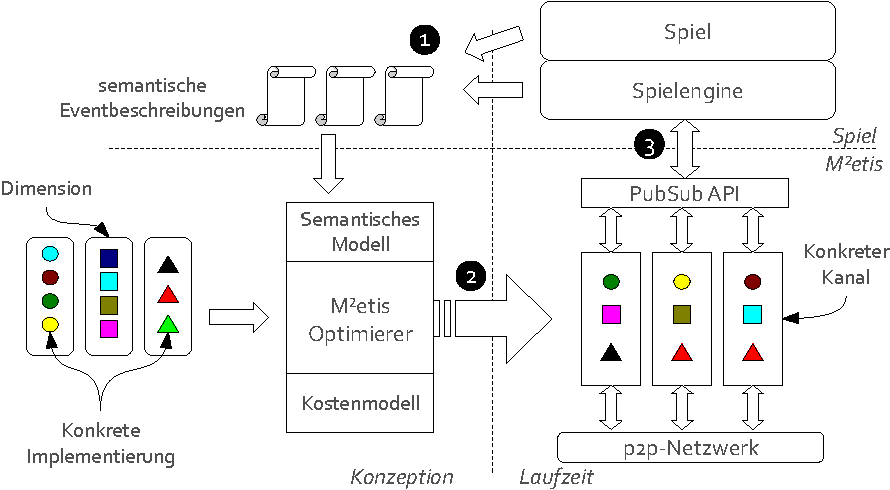
\includegraphics{grafics/metis_aufbau.pdf}}
\caption{Architekturübersicht von M$^2$etis}
\label{fig:metis_aufbau}
\end{figure}

\Fref{fig:metis_aufbau} zeigt die zeitliche Aufteilung des Systemes in \emph{Konzeption} und \emph{Laufzeit} sowie die Schnittpunkte von \ac{m2etis} mit dem \emph{Spiel}.

Im ersten Schritt werden die im Spiel genutzten Eventtypen durch den Spielentwickler identifiziert und semantisch beschrieben. Im zweiten Schritt verarbeitet der \ac{m2etis} \emph{Optimierer} diese Beschreibungen unter Zuhilfenahme des \emph{semantischen Modells} und des \emph{Kostenmodells}. Für jeden Typ wird dabei ein optimierter \emph{Kanal} erzeugt, in dem die unterschiedlichen Implementierungen der in \cite{Fischer2010a} beschriebenen Dimensionen Anwendung finden. Vom Benutzer implementierte Strategien, die mit entsprechenden Werten aus dem Kostenmodell versehen sind, werden von \ac{m2etis} im Optimierungslauf ebenfalls genutzt.\\
Die optimierte Kanäle lassen sich zur Laufzeit (im 3. Schritt) über die Publish/Subscribe-API ansprechen und kommunizieren über das \ac{p2p}-Netzwerk. Wie in der Grafik ersichtlich ist, benötigt das Spiel keine Implementierungsdetails der einzelnen Kanäle um diese zu nutzen.

Zuerst werden verschiedene \ac{p2p}-Netzwerke hinsichtlich ihres Einsatzes für \ac{m2etis} evaluiert. Weiterhin ist diese Arbeit für die Konzeption und prototypische Entwicklung des Publish/Subscribe-Systems sowie dessen Anbindung an das gewählte Netzwerk zuständig.\\
Damit das Framework frühzeitig einsetzbar ist, werden einige Algorithmen verschiedener Dimensionen implementiert. Die Entwicklung erfolgt wie vorgegeben in C++.
